\documentclass[12pt]{article}
\usepackage{graphicx} % Required for inserting images
\usepackage{indentfirst}
\usepackage[hyphens]{url}
\usepackage{hyperref}
\usepackage{tikz}
\usetikzlibrary{math}
\usepackage[section]{minted}
\usepackage{censor}
\usepackage{float}
\usepackage{amsthm}
\usepackage{amsmath,amssymb}
\usepackage{cleveref}
\usepackage[raggedright]{titlesec}
\usepackage{setspace}
\usepackage[numbib,nottoc]{tocbibind}
\usepackage[american]{babel}
\usepackage{natbib}
\usepackage{fancyhdr}
\usepackage{geometry}

\geometry{
 a4paper,
 left=1in,
 right=1in,
 top=1in,
 bottom=1in
}

\crefname{section}{Section}{Sections}
\crefname{figure}{Figure}{Figures}
\crefname{equation}{Equation}{Equations}
\creflabelformat{equation}{#2#1#3}

\newcommand{\Lagr}{\mathcal{L}}

\title{Using Lagrangian Mechanics\\ to solve the Double Pendulum}
\author{Saptak Das}
\date{November 2024}

% \onehalfspacing

\begin{document}

\maketitle

\section{Introduction}
The double pendulum is a classic problem in physics and nonlinear dynamics, offering a variety of complex behaviors ranging from regular periodic motion to chaotic trajectories. While Newtonian mechanics provides a straightforward framework for analyzing such systems, Lagrangian mechanics offers a more elegant and general approach, leveraging the principle of least action. This formulation simplifies the derivation of equations of motion for complex systems by focusing on energy rather than forces, making it particularly well-suited for systems with multiple degrees of freedom, like the double pendulum.

This paper presents a detailed analysis of the double pendulum using Lagrangian mechanics, beginning with the construction of the Lagrangian based on the system's kinetic and potential energy components. We then derive the equations of motion via the Euler-Lagrange equations, highlighting the advantages of this approach in reducing the complexity of the problem. Furthermore, the nonlinear nature of the equations is explored, shedding light on the chaotic dynamics that arise under certain initial conditions.

\section{Theoretical Background}
\subsection{Lagrangian Mechanics}
\noindent
The Lagrangian, \(\Lagr\), is defined as the difference between the system's kinetic energy, \(T\), and potential energy, \(U\):
\begin{equation}
    \Lagr = T - U
\end{equation}
\noindent
The equations of motion are derived using the Euler-Lagrange equation:
\begin{equation}
    \frac{d}{dt} \left( \frac{\partial L}{\partial \dot{q_i}}  \right) - \frac{\partial L}{\partial q_i} = 0
\end{equation}

\subsection{Double Pendulum}
\noindent
The double pendulum consists of two rods of lengths \(l_1\) and \(l_2\), with masses \(m_1\) and \(m_2\). The angular positions are described by \(\theta_1\) and \(\theta_2\), measured from the vertical.

\begin{figure}[H]
    \centering
    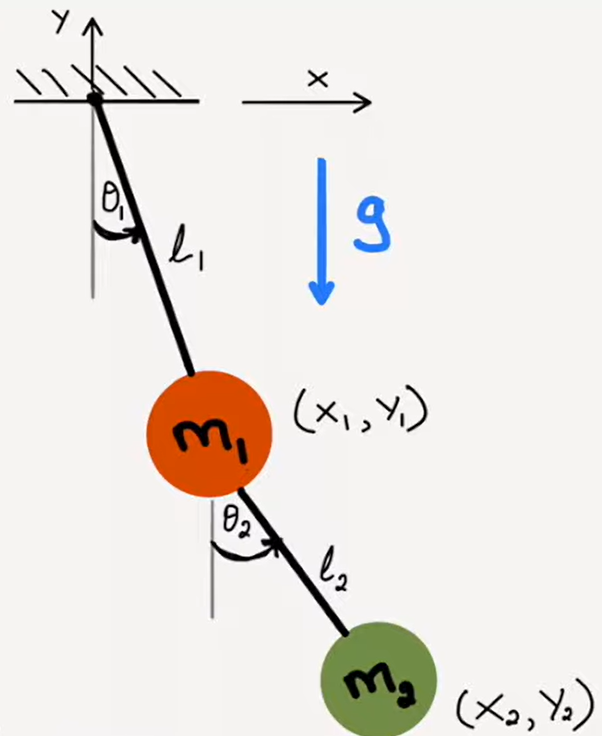
\includegraphics[width=70mm,height=\textheight,keepaspectratio]{images/double_pendulum.png}
    \caption{Diagram of Double Pendulum}
    \label{fig:double_pendulum}
\end{figure}

\section{Derivation}
\subsection{Kinematic Constraints}
\begin{align}
    x_1 &= l_1 \sin \theta_1 \\
    y_1 &= -l_1 \cos \theta_1 \\
    x_2 &= l_1 \sin \theta_1 + l_2 \sin \theta_2 \\
    y_2 &= -l_1 \cos \theta_1 - l_2 \cos \theta_2
\end{align}

\subsection{Velocities}
\begin{align}
    \dot{x_1} &= \dot{\theta_1} l_1 \cos \theta_1 \\
    \dot{y_1} &= \dot{\theta_1} l_1 \sin \theta_1 \\
    \dot{x_2} &= \dot{\theta_1} l_1 \cos \theta_1 + \dot{\theta_2} l_2 \cos \theta_2 \\
    \dot{y_2} &= \dot{\theta_1} l_1 \sin \theta_1 - \dot{\theta_2} l_2 \sin \theta_2
\end{align}

\subsection{Potential Energy}
\begin{align}
    U &= m_1 g y_1 + m_2 g y_2 \\
    &= -(m_1+m_2)g l_1 \cos \theta_1 - m_2 g l_2 \cos \theta_2
\end{align}

\subsection{Kinetic Energy}
\begin{align}
    T &= \frac{1}{2} m_1 v_1^2 + \frac{1}{2} m_2 v_2^2 \\
    &= \frac{1}{2} m_1 (\dot{x_1}^2 + \dot{y_1}^2) + \frac{1}{2} m_2 (\dot{x_2}^2 + \dot{y_2}^2) \\
    &= \frac{1}{2} m_1 l_1^2 \dot{\theta_1}^2 + \frac{1}{2} m_2 \left( l_1^2 \dot{\theta_1}^2 + l_2^2 \dot{\theta_2}^2 + 2 l_1 l_2 \dot{\theta_1} \dot{\theta_2} \cos (\theta_1 - \theta_2) \right)
\end{align}

\subsection{Lagrangian}
\begin{align}
    \Lagr &= T - V \\
    &= \frac{1}{2} m_1 l_1^2 \dot{\theta_1^2} + \frac{1}{2} m_2 \left( l_1^2 \dot{\theta_1^2} + l_2^2 \dot{\theta_2^2} + 2 l_1 l_2 \dot{\theta_1} \dot{\theta_2} \cos (\theta_1 - \theta_2) \right) \\
    &\qquad+ (m_1 + m_2) g l_1 \cos \theta_1 + m_2 g l_2 \cos \theta_2 \notag
\end{align}

\subsection{Euler-Lagrange Equation}
\begin{align}
    \frac{d}{dt} \left( \frac{\partial \Lagr}{\partial \dot{q}} \right) - \frac{\partial \Lagr}{\partial q} = 0
\end{align}

\subsubsection{Differential Equation Relation for \(\theta_1\)}
\begin{align}
    \frac{d}{dt} \left( \frac{\partial \Lagr}{\partial \dot{\theta_1}} \right) - \frac{\partial \Lagr}{\partial \theta_1} = 0
\end{align}
\begin{align}
    (m_1 + m_2) l_1 \ddot{\theta_1} + m_2 l_2 \ddot{\theta_2} \cos (\theta_1 - \theta_2) + m_2 l_2 \dot{\theta_2^2} \sin (\theta_1 - \theta_2) + (m_1 + m_2) g \sin \theta_1 = 0
\end{align}

\subsubsection{Differential Equation Relation for \(\theta_2\)}
\begin{align}
    \frac{d}{dt} \left( \frac{\partial \Lagr}{\partial \dot{\theta_2}} \right) - \frac{\partial \Lagr}{\partial \theta_2} = 0
\end{align}
\begin{align}
    m_2 l_2 \ddot{\theta_2} + m_2 l_1 \ddot{\theta_1} \cos (\theta_1 - \theta_2) - m_2 l_1 \dot{\theta_1^2} \sin (\theta_1 - \theta_2) + m_2 g \sin \theta_2 = 0
\end{align}

\section{Solution}
Though the nonlinear, coupled differential equations do not have an analytical solution, one can approximate the solution using numerical methods such as Runge-Kutta. The solution derived using an RK45 numerical integration is shown below.

\begin{figure}[H]
    \centering
    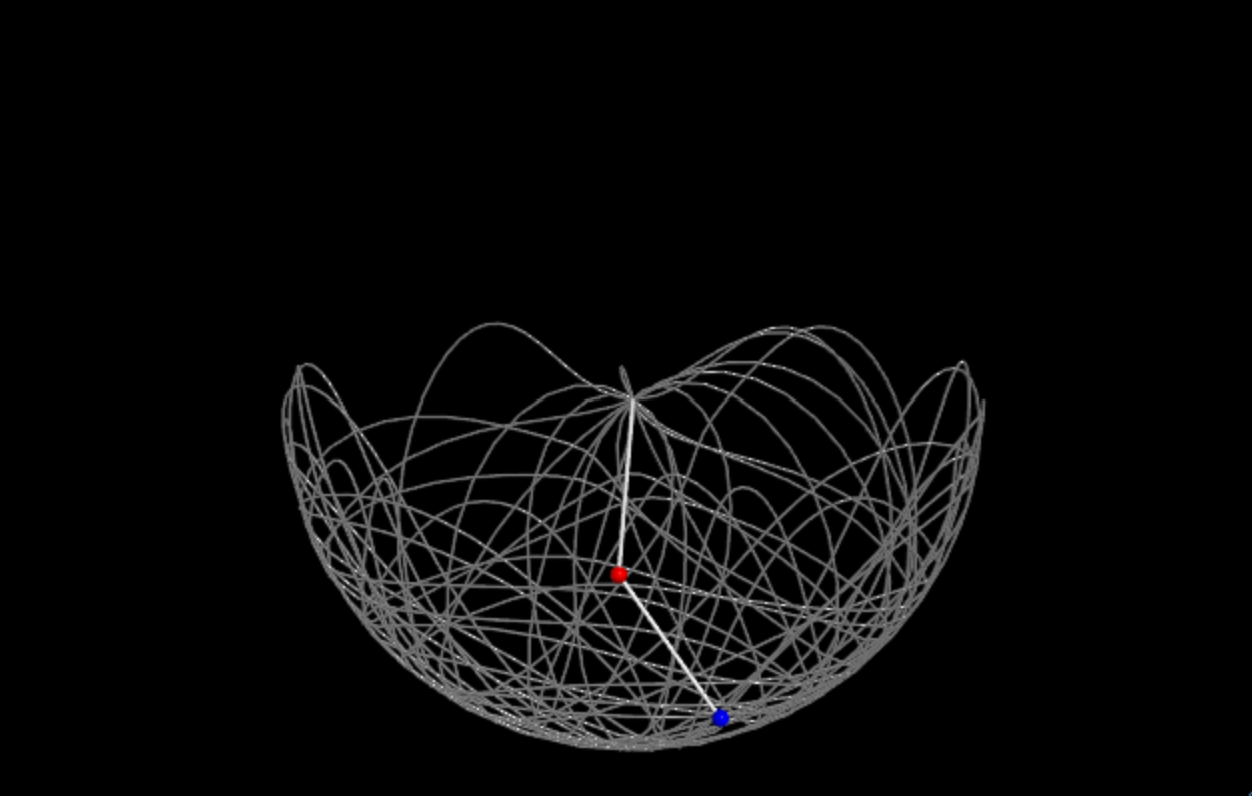
\includegraphics[width=70mm,height=\textheight,keepaspectratio]{images/double_pendulum_solution.png}
    \caption{Solution of a Double Pendulum using RK45 integration scheme as implemented in \url{https://www.glowscript.org/#/user/saptak.das625/folder/MyPrograms/program/Lab5DoublePendulum}}
    \label{fig:double_pendulum}
\end{figure}

\end{document}
